% PyCon US 2026 hallway poster v4
% Three-band conference-poster layout with integrated method visuals.

\documentclass[final]{beamer}

\usepackage[T1]{fontenc}
\usepackage{lmodern}
\usepackage[size=custom,width=120,height=72,scale=1.0]{beamerposter}
\usepackage{graphicx}
\usepackage{tikz}
\usepackage{xcolor}

\usetikzlibrary{arrows.meta,positioning}

\definecolor{paper}{HTML}{FFF8F2}
\definecolor{ink}{HTML}{17202A}
\definecolor{muted}{HTML}{5F6B74}
\definecolor{line}{HTML}{E2D6C8}
\definecolor{cityured}{HTML}{B01117}
\definecolor{cityumaroon}{HTML}{981B49}
\definecolor{cityuorange}{HTML}{E07541}
\definecolor{cpublue}{HTML}{1F7A8C}
\definecolor{validgreen}{HTML}{2F7D32}
\definecolor{a100berry}{HTML}{B51E59}
\definecolor{bandsoft}{HTML}{F9ECE5}
\definecolor{softblue}{HTML}{EAF2FB}
\definecolor{softgreen}{HTML}{EAF6EA}
\definecolor{softberry}{HTML}{F8E7EF}

\setbeamercolor{background canvas}{bg=paper}
\setbeamercolor{normal text}{fg=ink}
\setbeamertemplate{navigation symbols}{}
\setlength{\parindent}{0pt}
\hyphenpenalty=10000
\exhyphenpenalty=10000

\tikzset{
  flowstep/.style={
    rounded corners=0.12cm,
    fill=paper,
    draw=line,
    line width=0.06cm,
    inner sep=0.28cm,
    minimum width=20.7cm,
    minimum height=3.45cm,
    align=center,
    font=\fontsize{20}{23}\selectfont\bfseries,
    text=ink
  },
  flowarrow/.style={-{Latex[length=0.55cm,width=0.42cm]}, line width=0.11cm, draw=cityumaroon},
  badge/.style={
    rounded corners=0.12cm,
    inner sep=0.34cm,
    minimum width=9.2cm,
    minimum height=3.1cm,
    align=center,
    font=\fontsize{17}{20}\selectfont\bfseries
  }
}

\newcommand{\sectiontitle}[2]{%
  {\fontsize{31}{35}\selectfont\bfseries\color{cityured}#1\par}
  \vspace{0.16cm}
  {\fontsize{18}{21}\selectfont\bfseries\color{cpublue}#2\par}
}

\newcommand{\statement}[1]{%
  {\fontsize{19}{23}\selectfont\bfseries\color{ink}#1\par}
}

\newcommand{\tooltag}[2]{%
  \begingroup
  \setlength{\fboxsep}{0.36em}
  \colorbox{#1!12}{\fontsize{14}{17}\selectfont\bfseries\color{#1}#2}%
  \endgroup
}

\begin{document}
\begin{frame}[t]

% Background bands.
\begin{tikzpicture}[remember picture,overlay]
  \fill[paper] (current page.south west) rectangle (current page.north east);
  \fill[bandsoft] ([yshift=14.4cm]current page.south west) rectangle (current page.south east);
  \draw[cityured,line width=0.14cm] ([yshift=-13.1cm]current page.north west) -- ([yshift=-13.1cm]current page.north east);
  \draw[line,line width=0.05cm] ([yshift=14.4cm]current page.south west) -- ([yshift=14.4cm]current page.south east);
\end{tikzpicture}

% Band 1: Header / thesis.
\vspace{0.65cm}
\begin{columns}[c,totalwidth=0.94\paperwidth]
  \begin{column}{0.12\paperwidth}
    \centering
    
\includegraphics[width=0.82\linewidth]{cityu_logo.pdf}
  \end{column}
  \begin{column}{0.69\paperwidth}
    {\fontsize{78}{82}\selectfont\bfseries\color{cityumaroon}Breaking the Speed Limit\par}
    \vspace{0.22cm}
    {\fontsize{31}{36}\selectfont\bfseries\color{ink}Fast statistical models with Python 3.14, Numba, and JAX\par}
    \vspace{0.38cm}
    {\fontsize{28}{33}\selectfont\bfseries\color{ink}Simulation gives us an answer key when real data has no ground truth.\par}
    \vspace{0.18cm}
    {\fontsize{22}{26}\selectfont\bfseries\color{cityured}Validate first. Then accelerate the bottleneck.\par}
    \vspace{0.30cm}
    {\fontsize{16}{19}\selectfont\bfseries\color{cityumaroon}Wenxin Jiang \(\cdot\) Jian Yin\par}
    {\fontsize{14}{17}\selectfont\bfseries\color{cityured}Department of Biostatistics, City University of Hong Kong \(\cdot\) PyCon US 2026\par}
  \end{column}
  \begin{column}{0.13\paperwidth}
    \centering
    
\includegraphics[width=0.44\linewidth]{assets/repo_qr.png}\\[-0.08cm]
    {\fontsize{8.5}{10}\selectfont\bfseries\color{ink}github.com/LucaJiang/FastStatisticalModels4Python}
  \end{column}
\end{columns}

% Band 2: Main visual body.
\vspace{1.25cm}
\begin{columns}[t,totalwidth=0.94\paperwidth]
  \begin{column}{0.225\paperwidth}
    \sectiontitle{Why simulation?}{An answer key for code}
    \vspace{0.70cm}
    \begin{tikzpicture}
      \node[flowstep] (a) {No ground truth\\in real data};
      \node[flowstep,below=1.02cm of a] (b) {Simulate\\known behavior};
      \node[flowstep,below=1.02cm of b] (c) {Write readable\\reference};
      \node[flowstep,below=1.02cm of c] (d) {Check recovery\\calibration\\equivalence};
      \node[flowstep,below=1.02cm of d] (e) {Optimize\\the bottleneck};
      \draw[flowarrow] (a) -- (b);
      \draw[flowarrow] (b) -- (c);
      \draw[flowarrow] (c) -- (d);
      \draw[flowarrow] (d) -- (e);
    \end{tikzpicture}
    \vspace{0.82cm}
    \begingroup
      \setlength{\fboxsep}{0.48em}
      \colorbox{softgreen}{\begin{minipage}{0.88\linewidth}
        {\fontsize{20}{24}\selectfont\bfseries\color{validgreen}Speed only counts after the result matches the validation target.\par}
      \end{minipage}}
    \endgroup
  \end{column}

  \begin{column}{0.347\paperwidth}
    \sectiontitle{Workload 1: k-means}{Iterative model fitting: assign \(\rightarrow\) update \(\rightarrow\) repeat}
    \vspace{0.55cm}
    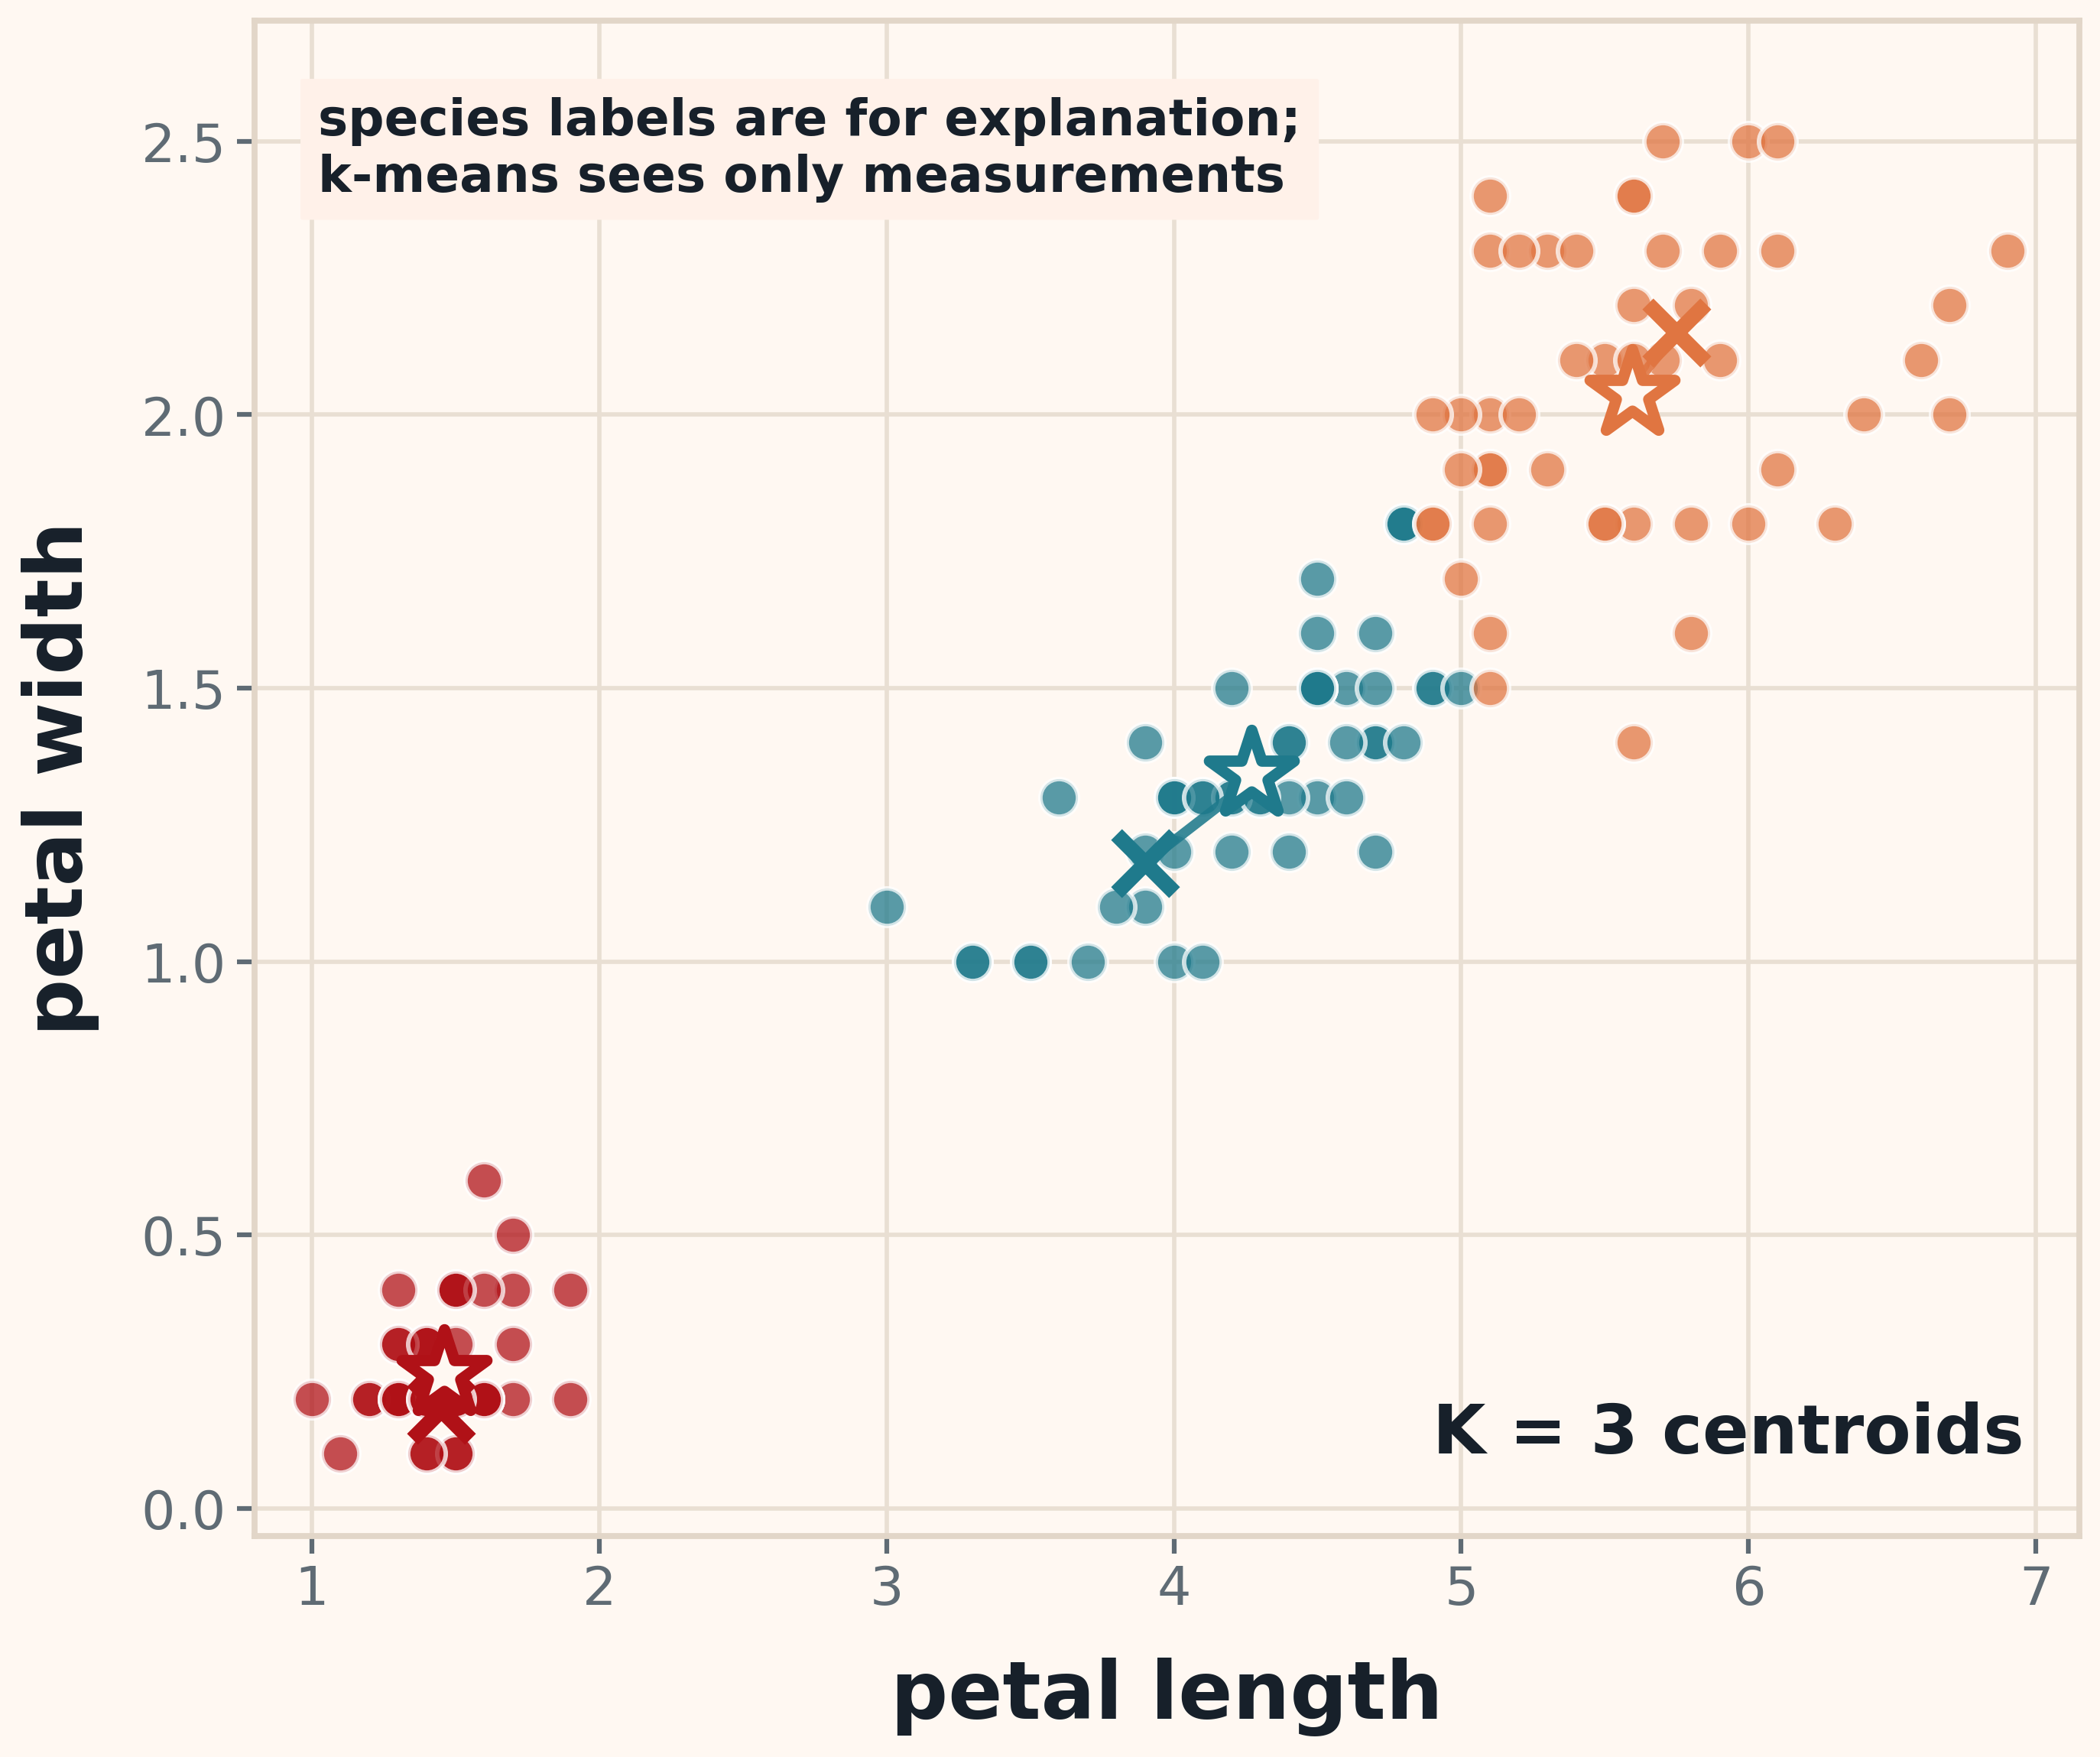
\includegraphics[width=\linewidth,height=35.0cm,keepaspectratio]{assets/poster_v4_kmeans_iris.png}
    \par\vspace{0.38cm}
    \begin{minipage}{\linewidth}
      \raggedright
      \statement{Same data and initialization.}
      \statement{Check recovery and final inertia.}
      \statement{Then compare implementations.}
      \vspace{0.44cm}
      \tooltag{validgreen}{Numba = loops}
      \hspace{0.16cm}
      \tooltag{cpublue}{NumPy/BLAS = distance algebra}
      \hspace{0.16cm}
      \tooltag{a100berry}{JAX/A100 = large regular arrays}
    \end{minipage}
  \end{column}

  \begin{column}{0.347\paperwidth}
    \sectiontitle{Workload 2: permutation test}{Resampling inference: shuffle \(\rightarrow\) statistic \(\rightarrow\) repeat}
    \vspace{0.55cm}
    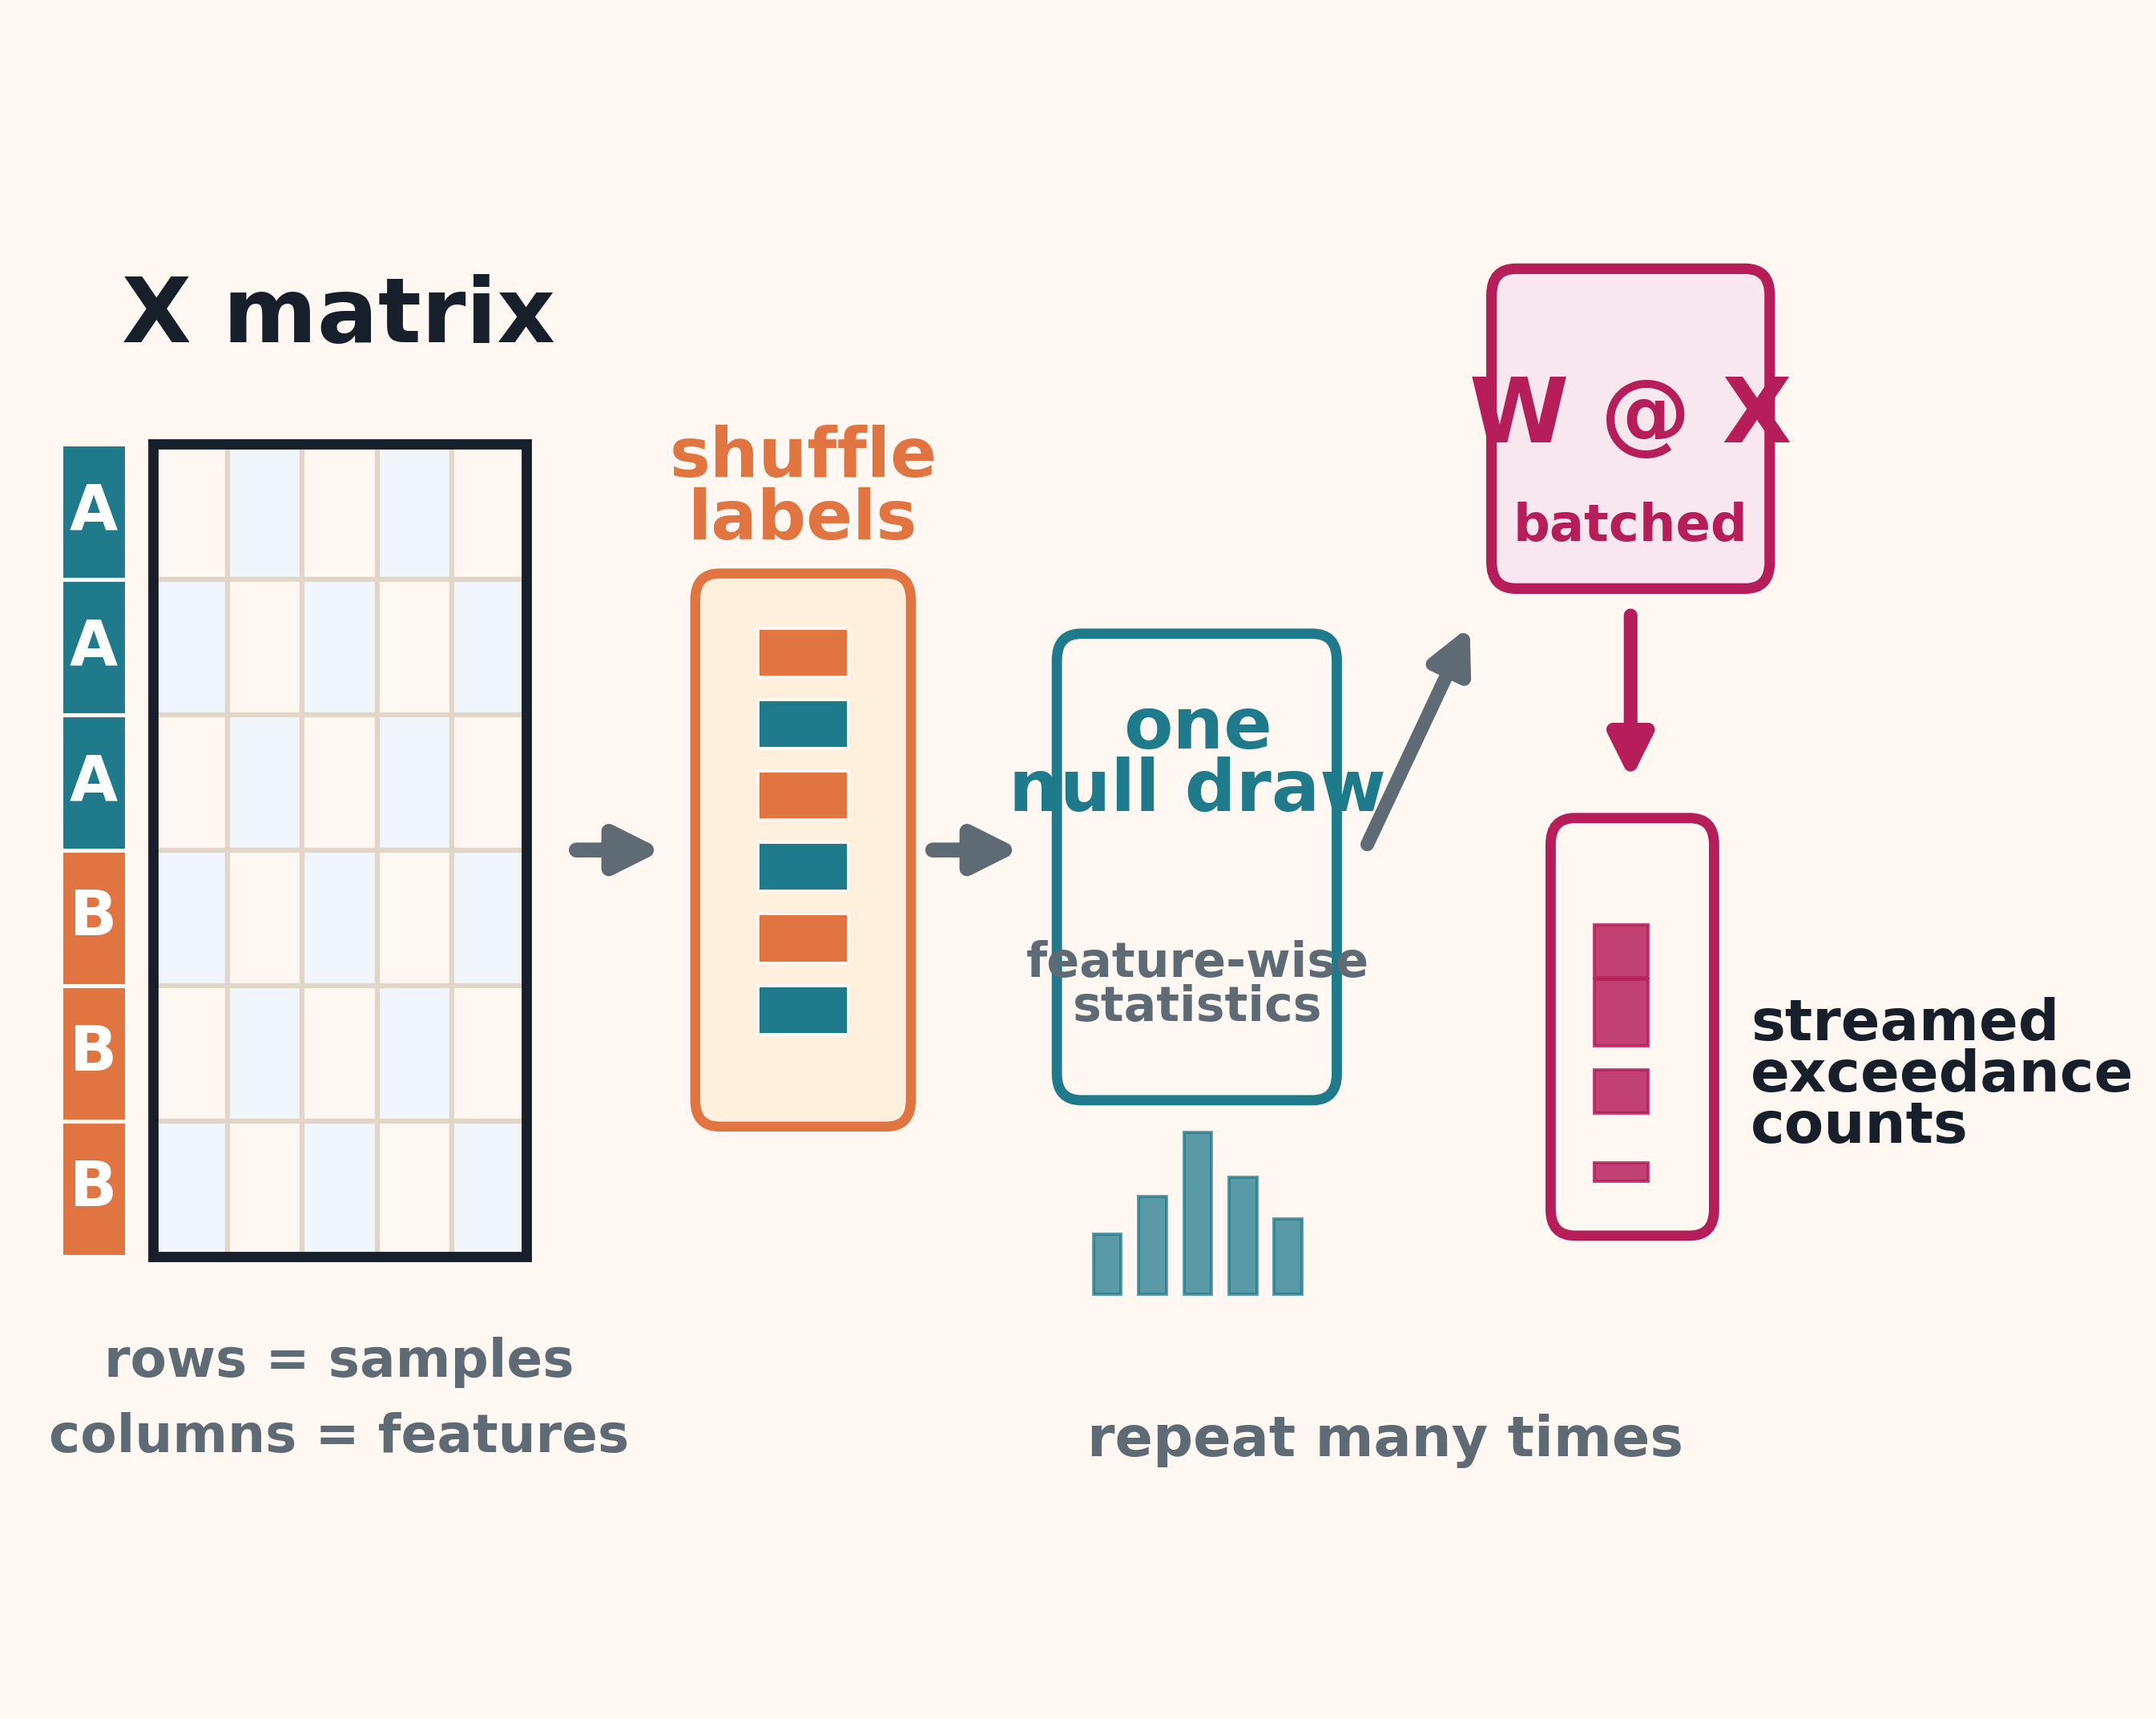
\includegraphics[width=\linewidth,height=35.0cm,keepaspectratio]{assets/poster_v4_permutation_workflow.png}
    \par\vspace{0.38cm}
    \begin{minipage}{\linewidth}
      \raggedright
      \statement{Same permutation stream.}
      \statement{Same p-value definition.}
      \statement{Check null calibration before timing.}
      \vspace{0.44cm}
      \begingroup
        \setlength{\fboxsep}{0.36em}
        \colorbox{softblue}{\fontsize{15}{18}\selectfont\bfseries\color{cpublue}CPU wins when overhead dominates.}
        \hspace{0.18cm}
        \colorbox{softberry}{\fontsize{15}{18}\selectfont\bfseries\color{a100berry}A100 helps when \(R \times p\) is large and the pipeline stays on device.}
      \endgroup
    \end{minipage}
  \end{column}
\end{columns}

% Band 3: Decision rule / evidence badges.
\vspace{0.80cm}
\begin{columns}[c,totalwidth=0.94\paperwidth]
  \begin{column}{0.64\paperwidth}
    {\fontsize{24}{28}\selectfont\bfseries\color{ink}
      Simulate known behavior
      \(\rightarrow\)
      Validate the result
      \(\rightarrow\)
      Identify the bottleneck
      \(\rightarrow\)
      Choose the smallest tool
      \par}
  \end{column}
  \begin{column}{0.30\paperwidth}
    \begin{tikzpicture}
      \node[badge,fill=softgreen,text=validgreen] at (0,0) {MacBook\\{\fontsize{13}{16}\selectfont validation and debugging}};
      \node[badge,fill=softblue,text=cpublue] at (10.2,0) {Linux server CPU\\{\fontsize{13}{16}\selectfont parallelism and memory}};
      \node[badge,fill=softberry,text=a100berry] at (20.4,0) {A100\\{\fontsize{13}{16}\selectfont batched device-resident workloads}};
    \end{tikzpicture}
  \end{column}
\end{columns}

\vspace{4.80cm}
\begin{center}
  {\fontsize{35}{40}\selectfont\bfseries\color{cityumaroon}Clear enough to trust. Fast enough to scale.\par}
\end{center}
\vspace{0.35cm}

\end{frame}
\end{document}
